\documentclass{article}
\usepackage[a4paper]{geometry}
\pagestyle{empty}
\newgeometry{margin=1cm}
\setlength{\parindent}{0pt}

% \usepackage[english,french]{babel}

\usepackage{style}
\usepackage{graphicx}
\usepackage{ragged2e}
\usepackage{hyperref}
\hypersetup{
    colorlinks=false,
    linkcolor=deepgray,
    filecolor=deepgray,
    urlcolor=deepgray,
    citecolor=deepgray,
    anchorcolor=deepgray,
    menucolor=deepgray,
    runcolor=deepgray,
    linkbordercolor={1 1 1}, % set to white
    filebordercolor={1 1 1},
    urlbordercolor={1 1 1},
    citebordercolor={1 1 1},
    pdfborder={0 0 0}
}
\usepackage{tikz}

\let\oldhrule\hrule
\renewcommand{\hrule}{\color{lightgray}\oldhrule\color{black}}
\makeatletter
\newcommand{\rubric}[1]{
    \color{mediumgray}
    \section*{\montserratlight \large \MakeUppercase{#1}} 
    \hrule
    \vspace{4mm}
    \raggedright
}

\begin{document}
% ================================== HEADER ===========================================
\begin{minipage}{0.35\textwidth}
  \begin{tikzpicture}
    \clip (0,0) circle (16mm);
    \node[xshift=-2mm, yshift=-2mm] at (0,0) {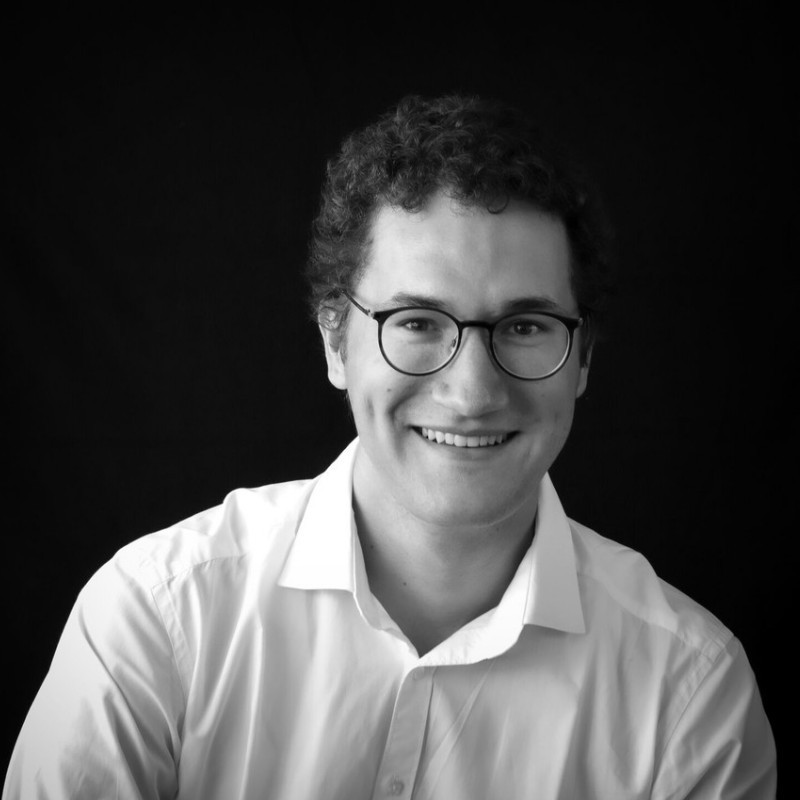
\includegraphics[width=4cm]{arnaud-cv}};
  \end{tikzpicture}
\end{minipage}
\begin{minipage}{0.65\textwidth}
  % \centering
  \montserratlight{\Huge ARNAUD  PANNATIER} \vspace{2mm}

  \sc \montserratthin Doctorat sur les modèles à attention et leurs applications
\end{minipage}
\vspace{4mm}
\hrule

% ==================================== INFO ============================================
\vspace{4mm}
\color{deepgray}
\small
Je suis doctorant au sein du groupe de Machine Learning du Pr. François Fleuret (Idiap Research Institute / EPFL). Mon principal centre d'intéret est sur les modèles à attention et leur adaptabilité à différents domaines allant de la prédiction du vent, l'aide au contrôle aérien, à la vision ou le traitement automatique du langage. Je travaille en collaboration étroite avec des entreprises sur des problèmes concrets avec des données réelles. \\
% ============================ Education & Publications ================================
\begin{minipage}[t]{0.3\textwidth}
  \rubric{Éducation}

  \color{deepgray}
  \large Doctorat en Machine Learning \\
  \color{mediumgray} \small
  Innosuisse, avec SkySoft ATM \\
  Idiap Research Institute / EPFL \\
  2020 - 2024

  \vspace{4mm}
  \color{deepgray}
  \large Master en Computer Sciences and Engineering \\
  \color{mediumgray} \small
  Faculté de Mathématiques, EPFL \\
  2017 - 2020

  \vspace{4mm}
  \color{deepgray}
  \large Bachelor en Physique \\
  \color{mediumgray} \small
  Faculté de Physique, EPFL \\
  2014 - 2017

\end{minipage}\hfill
\begin{minipage}[t]{0.65\textwidth}
  \rubric{Publications}
  \small
  A. Pannatier, K. Matoba, F. Fleuret \textbf{Inference from Real-World Sparse Measurements} \textit{under review at International Conference on Learning Representations (ICLR), 2024}
  \vspace{4mm}

  F. Mai, A. Pannatier, F. Fehr, H. Chen, F. Marelli, F. Fleuret, J. Henderson \textbf{HyperMixer: An MLP-based Low Cost Alternative to Transformers.} In \textit{Proceedings of the Annual Meeting of the Association for Computational Linguistics (ACL), 2023.}
  \vspace{4mm}

  A. Pannatier, R. Picatoste, and F. Fleuret. \textbf{Efficient Wind Speed Nowcasting with GPU-Accelerated Nearest Neighbors Algorithm.} In \textit{Proceedings of the SIAM International Conference on Data Mining (SDM), 2022.}
  \vspace{4mm}

  A. Pannatier \textbf{A Control Plane in Time and Space for Locality-Preserving Blockchains} In \textit{Master Thesis, Decentralized Distributed Systems Laboratory (DEDIS), EPFL, 2020} \\
  \textbf{Prix: Kudelski Award}
  \vspace{4mm}
\end{minipage}
% ============================ Language & Experience ================================

\begin{minipage}[t]{0.3\textwidth}

  \rubric{Langues}
  \color{deepgray}
  \small
  \begin{tabular}{@{}ll@{}}
    Français:  & Langue maternelle     \\
    Anglais:   & Courant               \\
    Allemand : & Connaissances de base
  \end{tabular}

\end{minipage}\hfill
\begin{minipage}[t]{0.65\textwidth}

  \rubric{Expérience en Enseignement}

  \color{deepgray}
  \large Assistant
  \color{mediumgray} \small
  \begin{itemize}
    \item \color{deepgray}Analyse Avancée 1-2 \color{mediumgray} Pr. Stubbe, 2016, 2017, 2018
    \item \color{deepgray}Analyse 2 \color{mediumgray} Pr Buffoni, 2018
    \item \color{deepgray}Analyse Avancée 3 \color{mediumgray} Pr. Krieger, 2018
    \item \color{deepgray}Introduction à l'apprentissage automatique  \color{mediumgray} Pr. Liebling, 2020, 2023
    \item \color{deepgray}Deep Learning \color{mediumgray} Pr. Fleuret, 2021, 2022
    \item \color{deepgray}Information, Computation, Communication  \color{mediumgray} Pr. Chappelier, 2020, 2022, 2023
  \end{itemize}

  \vspace{4mm}
  \color{deepgray}
  \large Remplacements \\
  \color{mediumgray} \small
  Lycée Collège de la Planta \\
  2019
  \rubric{Expérience professionnelle}

  \color{deepgray}
  \large Ingénieur logiciel \\
  \color{mediumgray} \small
  Caelum Fintech SA, Technopôle \\
  2018 - 2020 (à temps partiel)
  \vspace{4mm}
\end{minipage}
% ============================ Info & Interests ================================

\begin{minipage}[t]{0.3\textwidth}
  \rubric{Informations}

  \color{deepgray} \small
  Rue des Longs-Prés 40 \\
  3960 Sierre \\

  \href{tel:+41774393016}{+41 77 439 30 16} \\
  \href{mailto:arnaud.pannatier@idiap.ch}{arnaud.pannatier@idiap.ch} \\
  \href{https://arnaudpannatier.ch}{https://arnaudpannatier.ch}  \\

  \vspace{4mm}

  Né le 20 septembre 1995, à Sion, Valais \\
  Marié, deux enfants (nés en 2022, 2023)

\end{minipage}\hfill
\begin{minipage}[t]{0.65\textwidth}
  \rubric{Intérêts}
  \normalsize
  \color{deepgray}
  Randonnée \\
  \color{mediumgray} \small
  Randonnée depuis le Valais jusqu'à Saint-Jacques-de-Compostelle (Espagne) \\
  2300 km en 83 jours (avril 2019 - juillet 2019)
  \vspace{3mm}

  \color{deepgray}
  \normalsize
  Échecs \\
  \color{mediumgray} \small
  Trésorier de l'Union Valaisanne des Échecs (UVE-WSB) \\
  Joue avec Sion 1 (1re ligue, précédemment Ligue B) \\
  Ancien capitaine de l'équipe d'échecs Valais 2 (2e ligue)
\end{minipage}

\end{document}